%% chapter 4 Species-level traits - responses to land use and climate-change sensititivy

\section*{Keywords}

\section*{Abstract}

\section{Introduction}

%% Figure 1 = framework

\begin{figure}[h!]
\centering
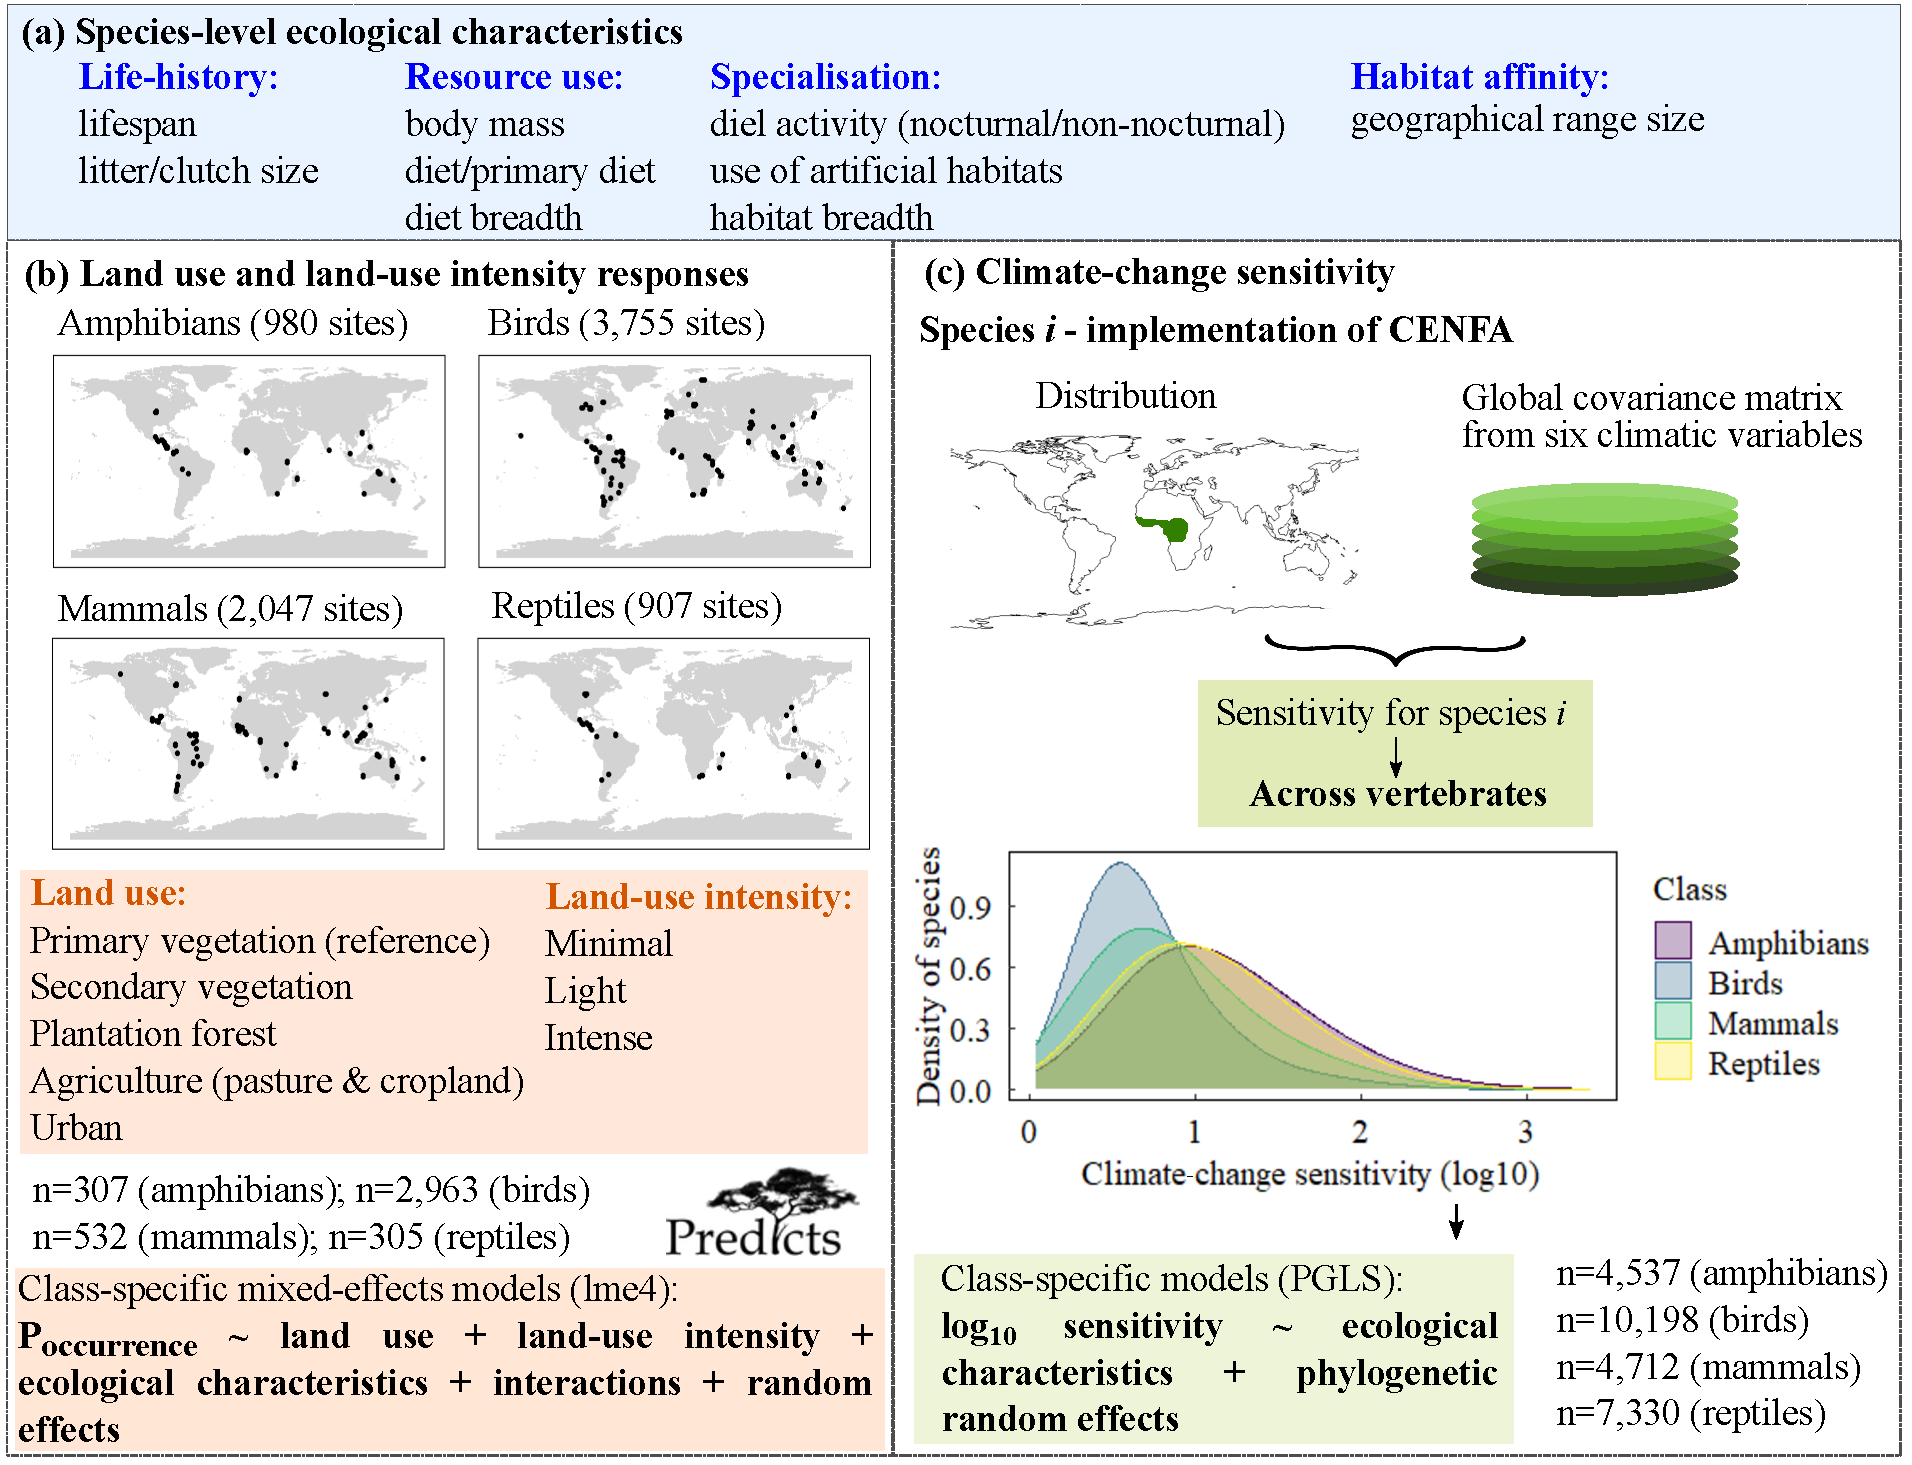
\includegraphics[scale=0.55]{figures/Chapter4/Figure1}
\caption[Framework of the study]{\textbf{Framework of the study.} \textbf{(a)} I collected ecological trait data and geographical range areas across terrestrial vertebrates (termed `ecological characteristics'). I then used two independent approaches to assess the influence of these characteristics on species responses to land-use and on species climate-change sensitivity. \textbf{(b)} To assess the influence of traits on responses to land use and land-use intensity in each vertebrate class, I combined the ecological characteristics with the PREDICTS database. \textbf{(c)} To estimate species sensitivity to climate change, I used the CENFA framework \citep{Rinnan2019}, which relies on the combination of species’ distributions with climatic variables to estimate sensitivity from properties of the species’ climatic niche space. I then built class-specific models to assess whether the ecological characteristics were associated with  species sensitivity to climate change.}
\label{chap4_fig1}
\end{figure}

\clearpage

\section{Methods}

%% Figure 2 = assessing effects 
\begin{figure}[h!]
\centering
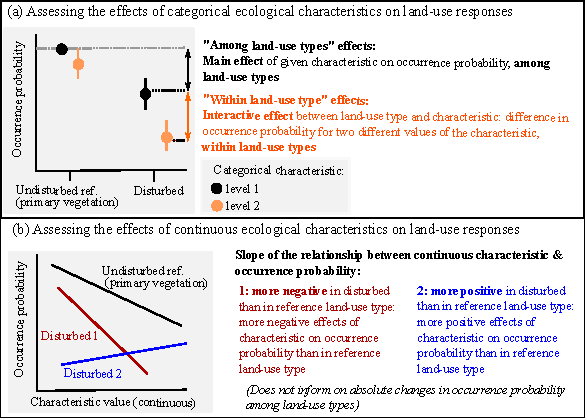
\includegraphics[scale=1.6]{figures/Chapter4/Figure2}
\caption[Assessing the effects of ecological characteristics on species land-use responses: methodology for (a) categorical characteristics and (b) continuous characteristics.]{\textbf{Assessing the effects of ecological characteristics on species land-use responses: methodology for (a) categorical characteristics and (b) continuous characteristics.} (a) For all categorical characteristics, except diet, I look at `within land-use type' effects, asking whether there are significant differences in occurrence probability between different functional groups in a given land-use type. For diet, I look at `among land-use type' effects, comparing species occurrence probability in disturbed land uses versus that in primary vegetation  (I chose this approach here because visualising `within land-use type' effects for diet is complicated by the fact that there are more than two levels for this categorical trait). (b) For continuous characteristics, I focus on the relationship with occurrence probability, and I investigate how the slope of this relationship is affected by land-use type. }
\label{chap4_fig2}
\end{figure}


\section{Results}


%% Synthesis table 
\begin{landscape}
\begin{table}[h!]
\centering
\caption[Summary of the effects of the ecological characteristics (except for primary diet) on species responses to disturbed land uses (`within land-use type' effects) and on species climate-change sensitivity, for each Class of terrestrial vertebrates.]{\textbf{Summary of the effects of the ecological characteristics (except for primary diet) on (a) species responses to disturbed land uses (`within land-use type' effects) and on (b) species climate-change sensitivity, for each class of terrestrial vertebrates.} The symbol \colorbox{Salmon}{\textcolor{BrickRed}{\textbf{--}}} indicates where a characteristic has a significant negative effect on occurrence probability within a disturbed land-use type, or where the characteristic renders species significantly more sensitive to climate change. A \colorbox{YellowGreen}{\textcolor{ForestGreen}{\textbf{+}}} indicates a significantly  positive effect of a characteristic on occurrence probability in a land-use type, or significantly lower sensitivity to climate change. For the land-use effects, we report `within land-use type effects' here, that is, within a disturbed land use whether there were significant differences in occurrence probability among species with different trait values (see Figure \ref{chap4_fig2}). These effects were derived from the interactive terms of the full, all-predictor models. I report effects detected in any land-use intensity.}
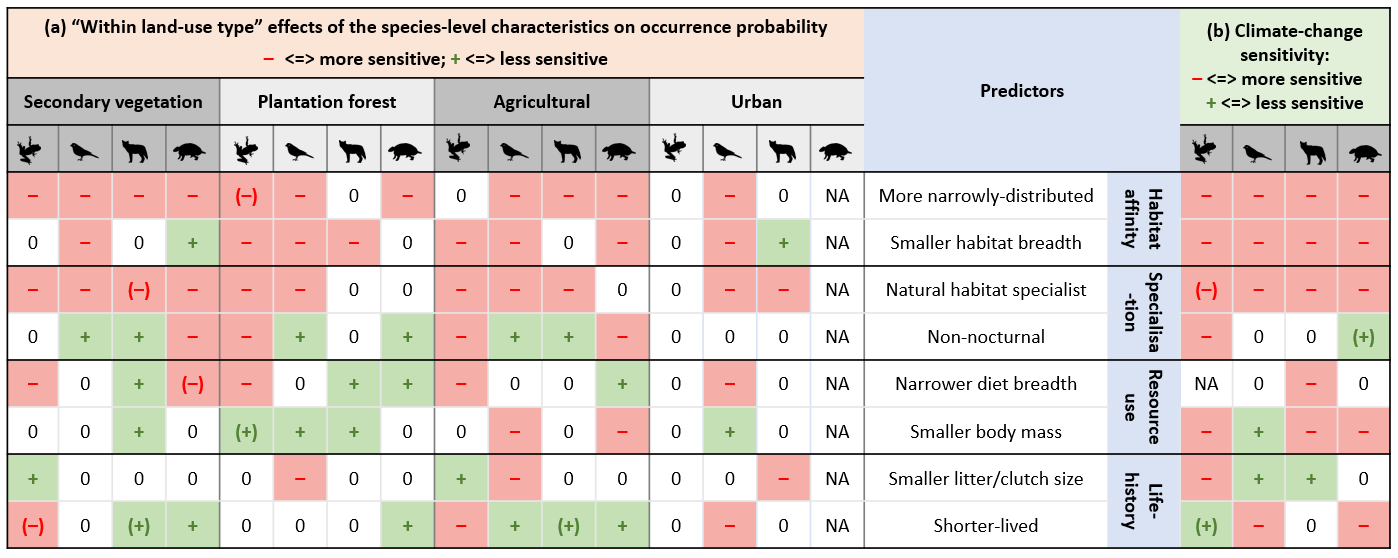
\includegraphics[scale=0.8]{figures/Chapter4/Synthesis_table}
\label{chap4_table1}
\end{table}
\end{landscape}


%% Diet figure
\begin{figure}[h!]
\centering
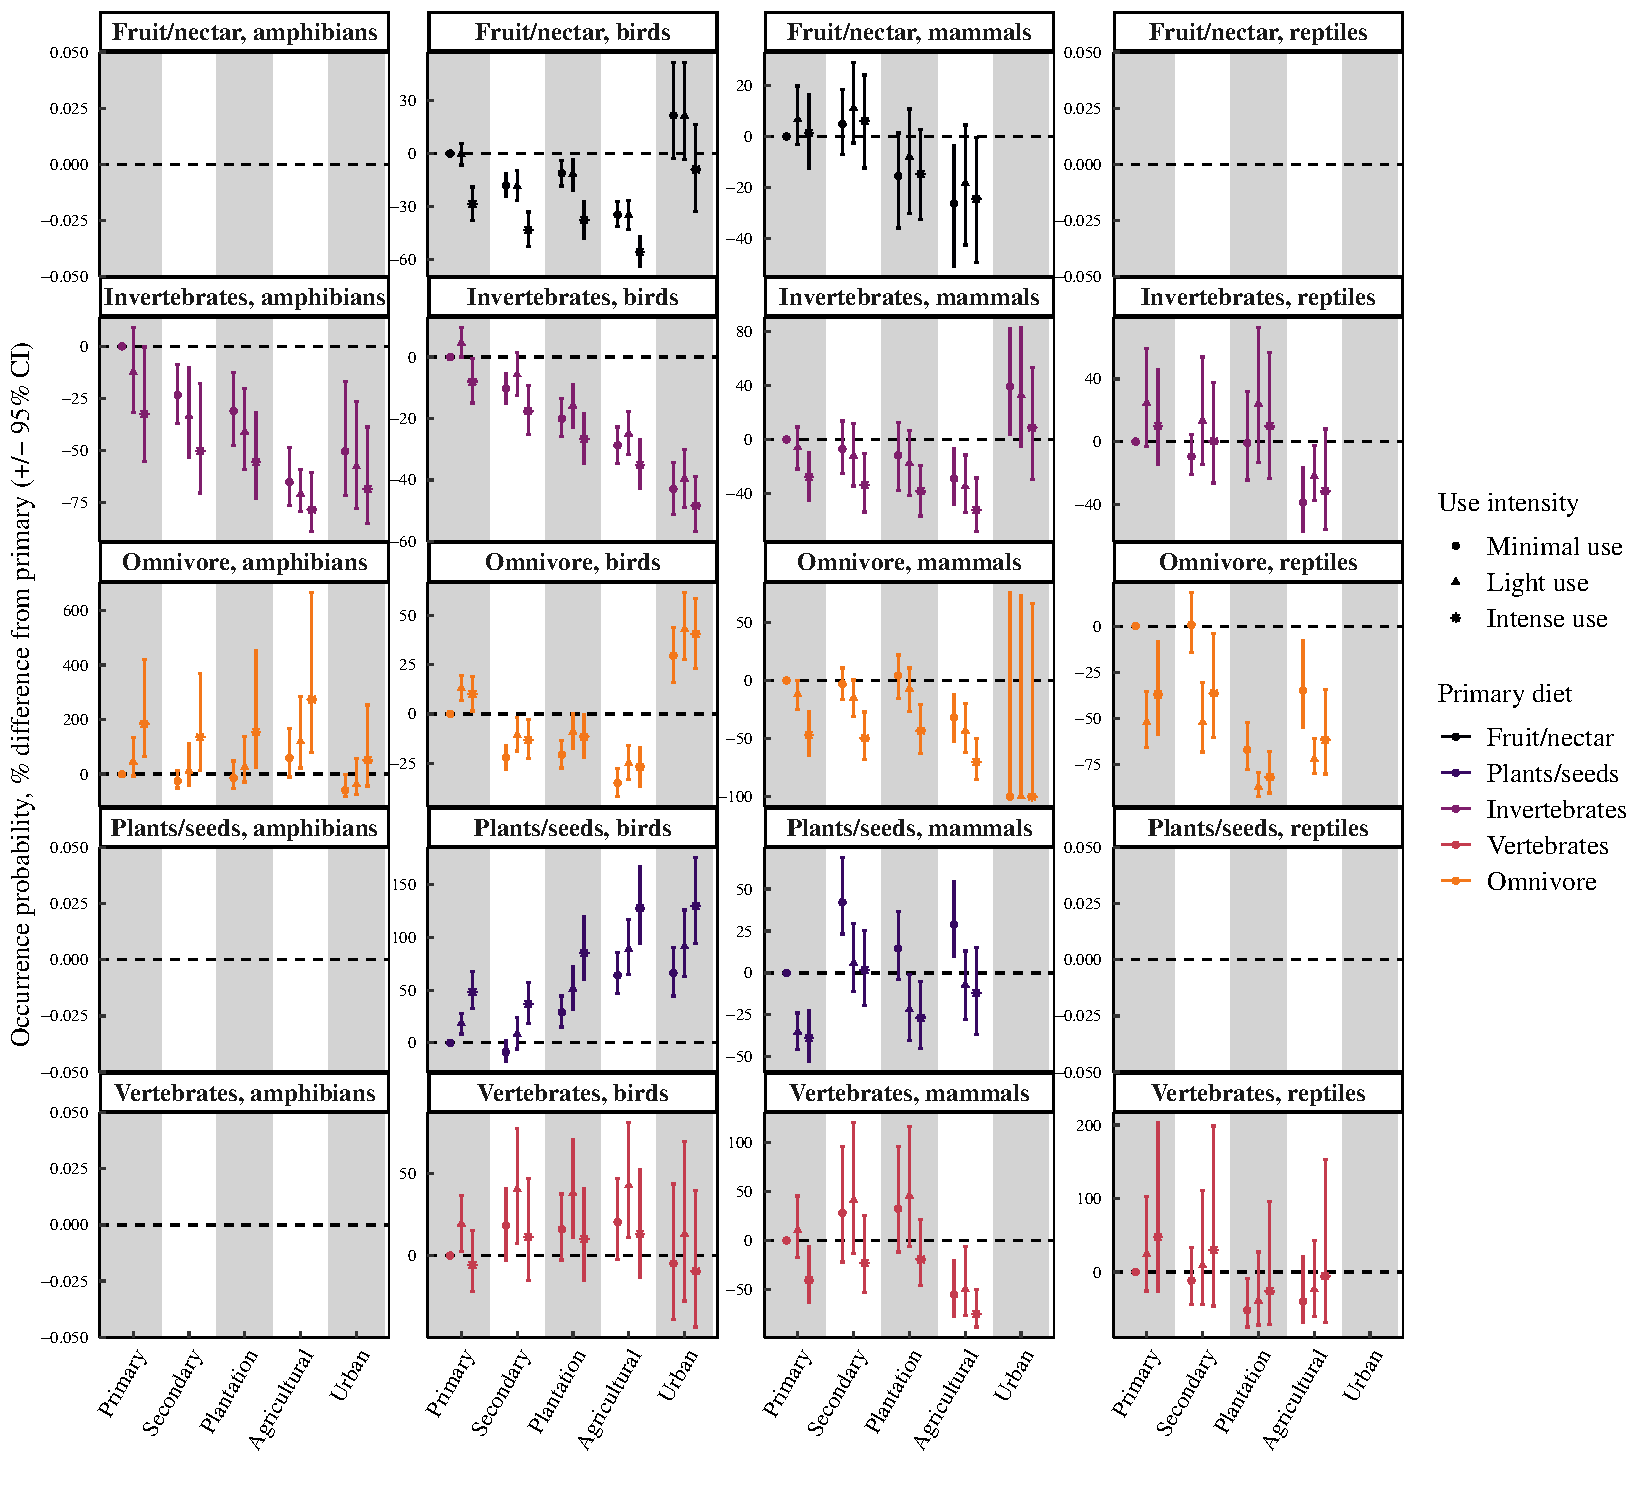
\includegraphics[scale=0.65]{figures/Chapter4/Figure3}
\caption[Predicted occurrence probability as a function of land use, land-use intensity, diet and their interactions, for each class of terrestrial vertebrates.]{\textbf{Predicted occurrence probability as a function of land use, land-use intensity, diet and their interactions, for each class of terrestrial vertebrates.} The predictions were obtained from the partial models fitted for each class considering only the diet trait. Empty plots are drawn where there were no data for a diet category for a given Class (e.g., amphibian fruit/nectar eaters). Effects could not be estimated for urban reptiles, as well as for urban vertebrate, fruit/nectar and plant/seed eaters for mammals because there were no sampled species. The predictions are rescaled with reference to minimally-used primary vegetation. Primary: primary vegetation; Secondary: secondary vegetation; plantation: plantation forest; agricultural: cropland and pasture.}
\label{chap4_fig3}
\end{figure}


%% Figure Variance
\begin{figure}[h!]
\centering
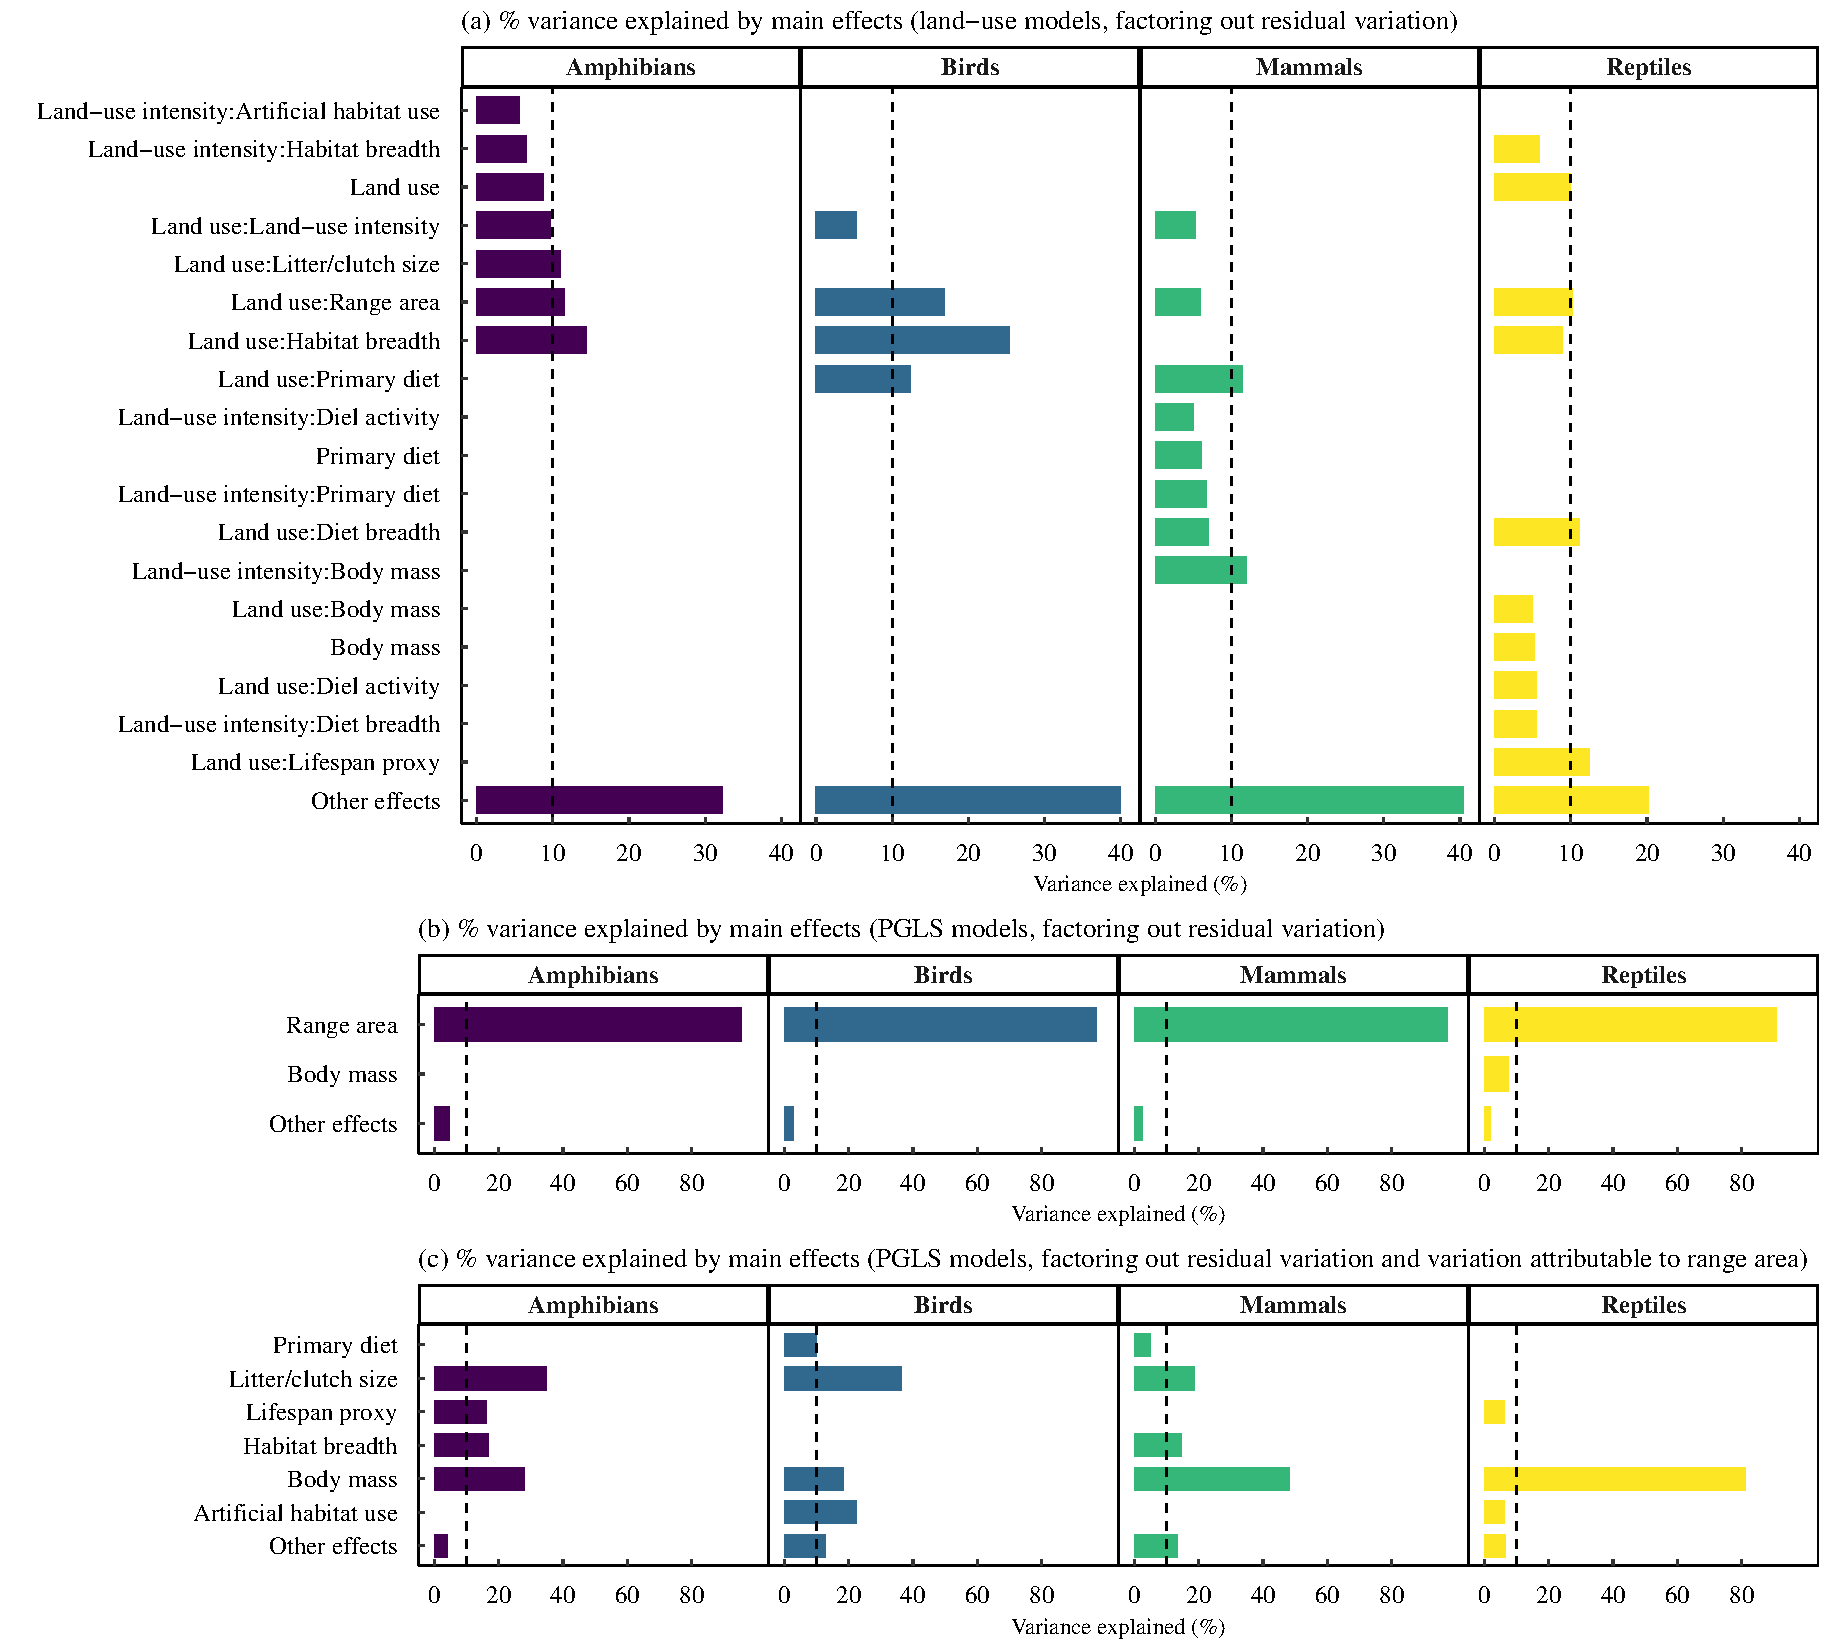
\includegraphics[scale=0.6]{figures/Chapter4/Figure4}
\caption[Proportion of the explained variance attributable to each of the main effects in the land-use and climate-change sensitivity models]{\textbf{Proportion of the explained variance attributable to each of the main effects} for (a) the mixed-effects models looking at the effects of land use, land-use intensity, and ecological characteristics on species occurrence probability (after factoring out residual variation); (b) for the phylogenetic least-squares regressions investigating whether the ecological characteristics explained climate-change sensitivity (after factoring out residual variation); (c) for the phylogenetic least-squares regressions investigating whether the ecological characteristics explained climate-change sensitivity (after factoring out the variance explained by geographical rage area and the residual variation). The dashed vertical lines mark 10\% explained variance. We individually show all the effects that explain more than 5\% of the overall variation. Effects that individually explain less than 5\% of the overall variation are grouped together as "Other effects".}
\label{chap4_fig4}
\end{figure}

%% Figure climate-change sensitivity - categorical predictors
\begin{figure}[h!]
\centering
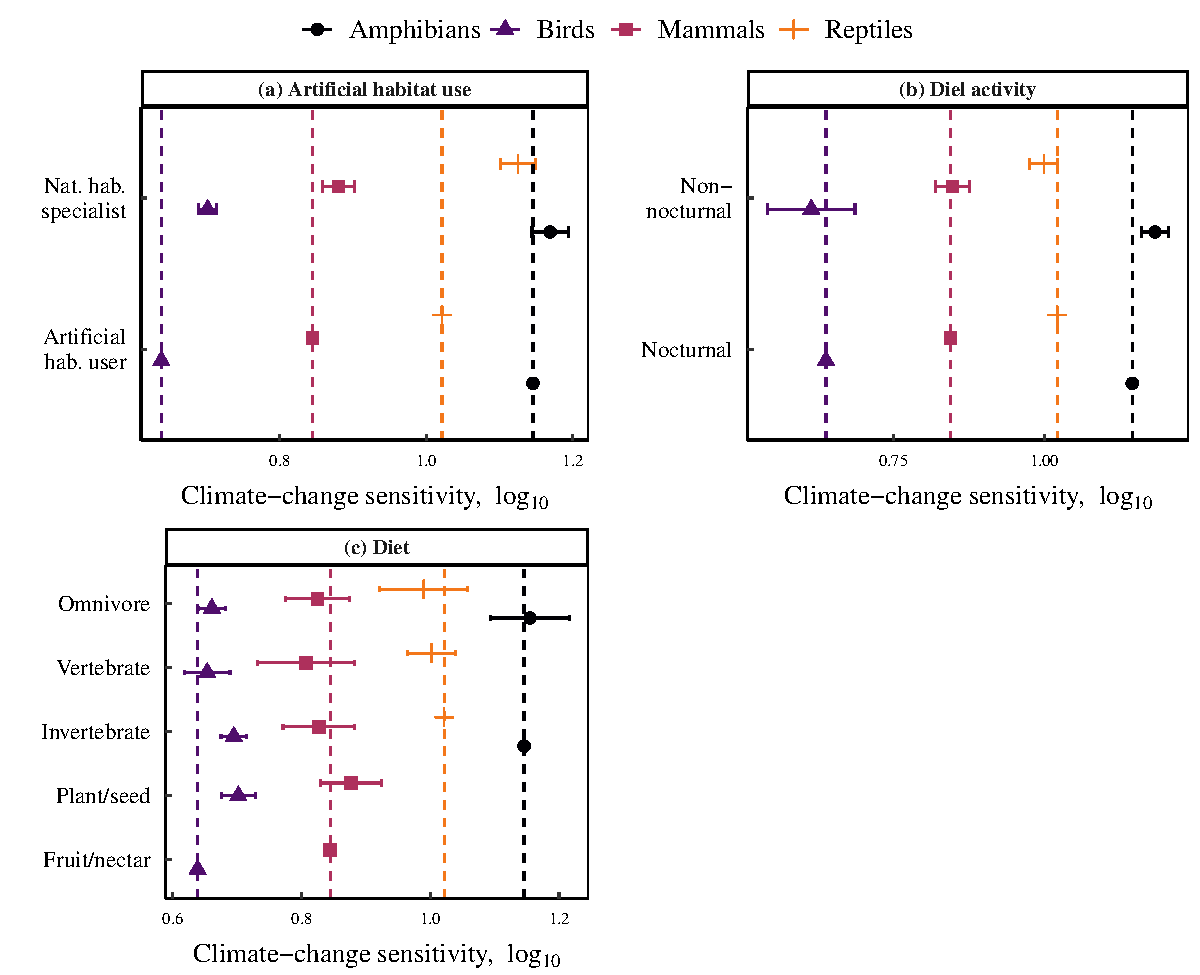
\includegraphics[scale=0.7]{figures/Chapter4/Figure5}
\caption[Effects of the categorical traits on climate-change sensitivity, estimated from the PGLS models in each class.]{\textbf{Effects of the categorical traits on climate-change sensitivity, estimated from the PGLS models in each class.} For artificial habitat use (a), the reference level is “artificial habitat user”; for diel activity, the reference level is “nocturnal”; for diet, the reference level for mammals and birds is “fruit/nectar eaters”, but “invertebrate eaters” for amphibians and reptiles. }
\label{chap4_fig5}
\end{figure}


%% Figure climate-change sensitivity - continuous predictors
\begin{figure}[h!]
\centering
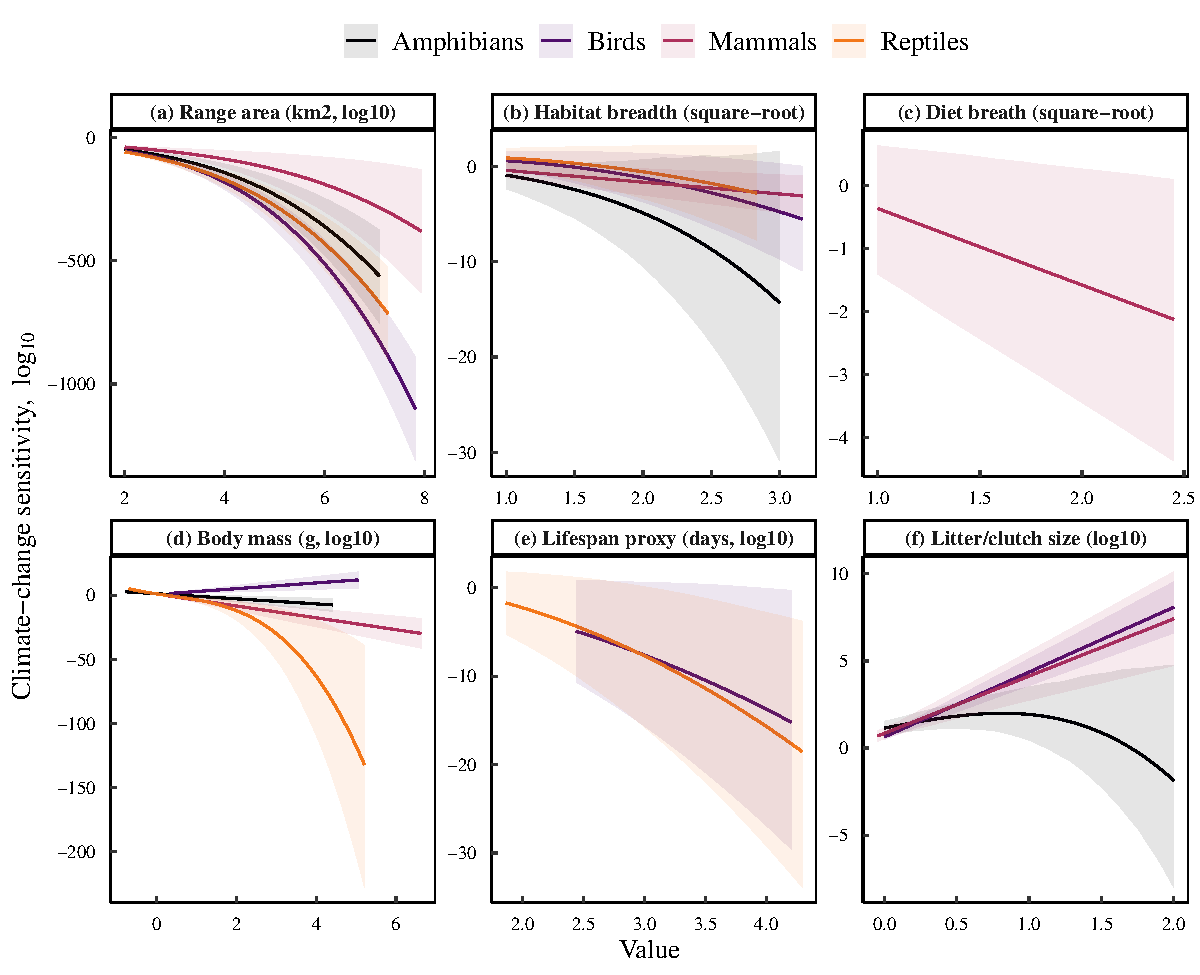
\includegraphics[scale=0.7]{figures/Chapter4/Figure6}
\caption[Effects of the continuous ecological characteristics on climate-change sensitivity, estimated from the PGLS models in each class.]{\textbf{Effects of the continuous ecological characteristics on climate-change sensitivity, estimated from the PGLS models in each class.} We plotted the estimated relationships only when they were found to be significant. }
\label{chap4_fig6}
\end{figure}


%% ANOVA table for PGLS models
\begin{table}[h!]
\centering
\caption[ANOVA summaries for the PGLS models investigating the effects of the species-level ecological characteristics on species climate-change sensitivity.]{\textbf{ANOVA summaries for the PGLS models investigating the effects of the species-level ecological characteristics on species climate-change sensitivity.}}
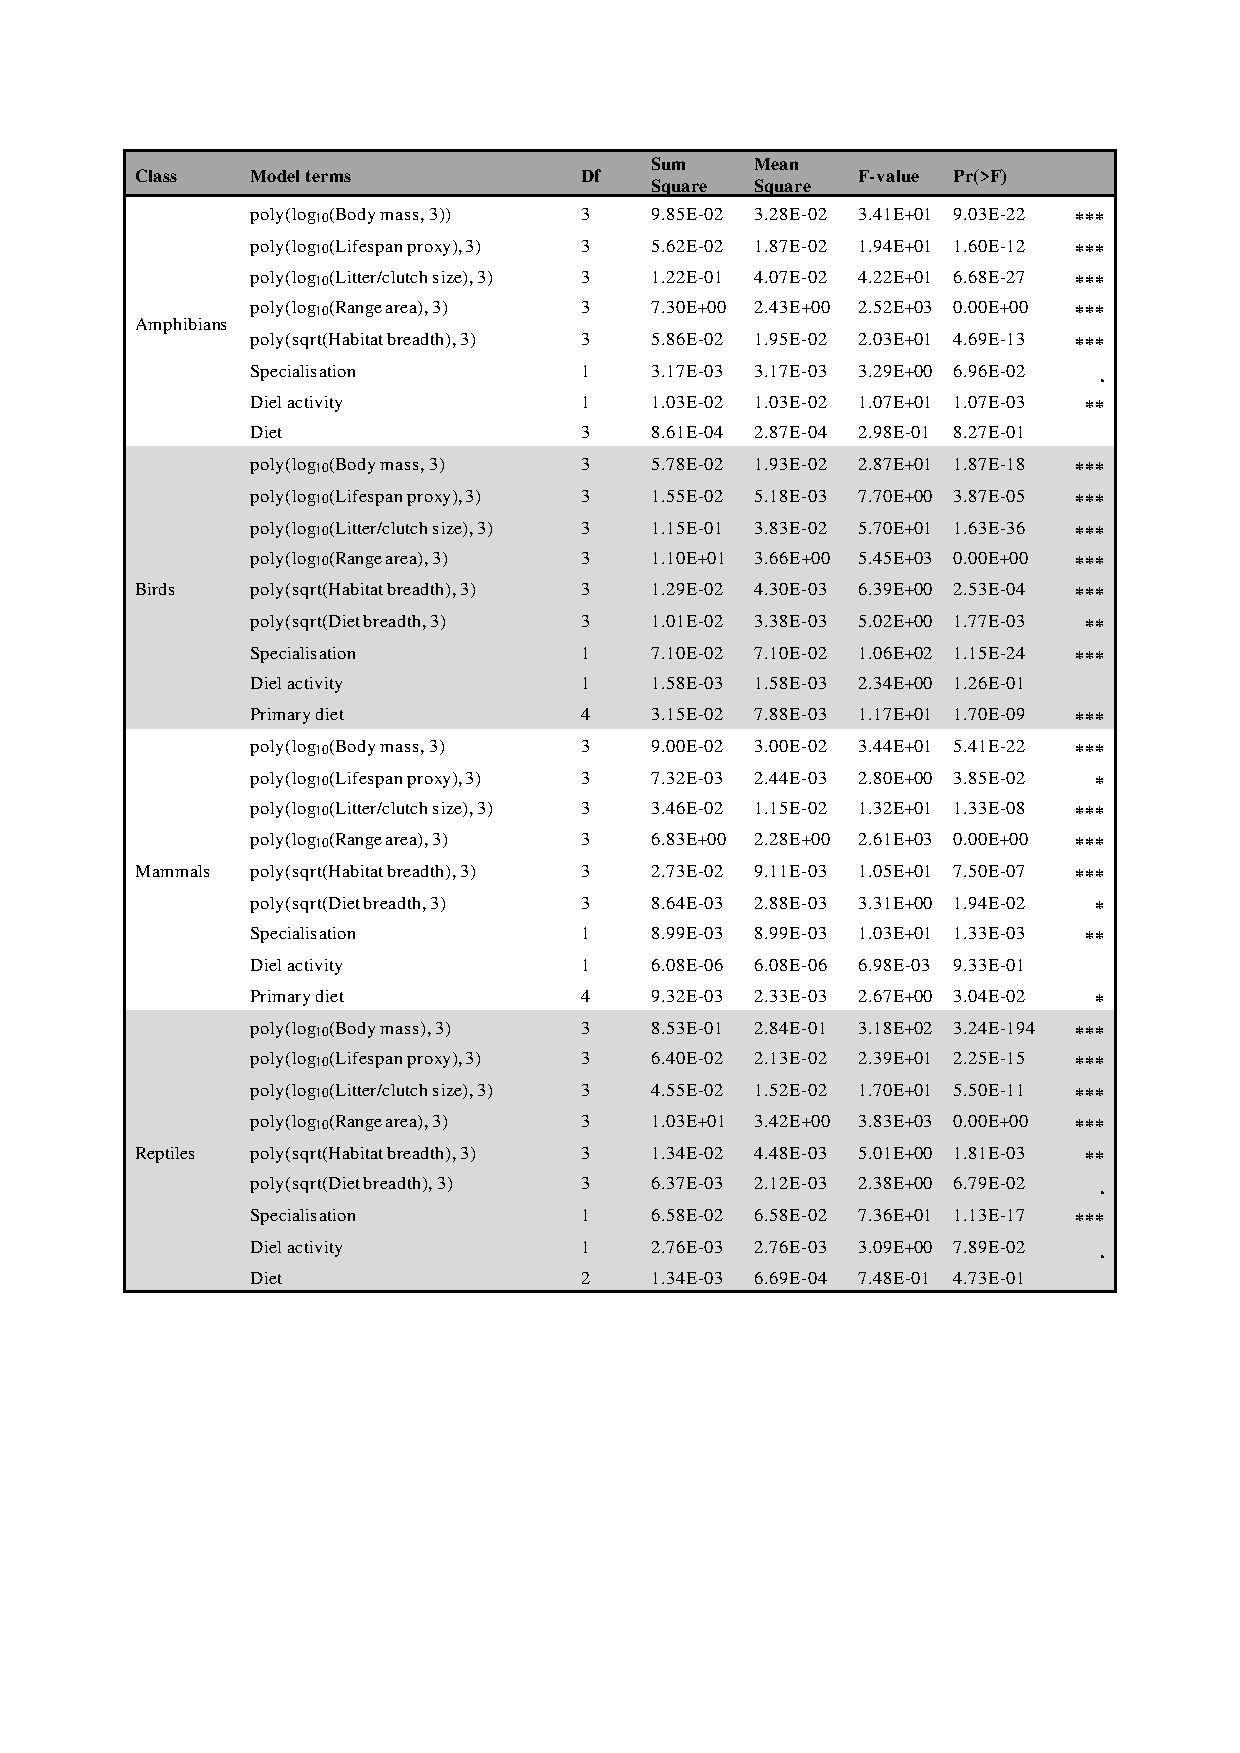
\includegraphics[scale=1, trim={2cm 5 1 2cm}, clip]{figures/Chapter4/Table_ANOVA_PGLS_pdf}
\label{chap4_table2}
\end{table}


\clearpage

\section{Discussion}
